\section{Modeling Methodology}
\label{sec:model}

This paper places considerable emphasis not only on the specific methods used but also on the process to select these methods, informed through a lens of MDO and systems thinking, with the intent to guide readers interested in conducting their own multidisciplinary WEC optimization.
In section~\ref{sec:model-overview}, the research objective and design scope are first used to define a broad problem formulation and module decomposition.
Next, section~\ref{sec:modules} describes the construction of the simulation model.
It develops the assumptions, analysis method, and implementation details of each module based on the appropriate balance of accuracy and speed.
Sections \ref{sec:validation} and \ref{sec:sim-runtime} discuss model validation and runtime benchmarking.
The simulation capabilities and limitations are then combined with the original broad design optimization intent to inform a detailed optimization problem formulation.
In this step, the exact objectives, design variables, constraints, and parameters are selected and outlined in section~\ref{sec:formulation}.
The resulting optimization problem is then characterized and its properties ultimately inform the solution method including algorithm selection, discussed in section~\ref{sec:optim-process}.
Finally, the process is tweaked iteratively until it yields satisfactory results, with noteworthy insights integrated into the relevant sections \ref{sec:model-overview} to \ref{sec:optim-process}.
Figure~\ref{fig:overview-methods} depicts this methodology visually.
\begin{figure}
    \centering
    \includegraphics[width=1\linewidth]{\matlabFilepath{2}}
    \caption{Methodology overview}
    \label{fig:overview-methods}
\end{figure}

\subsection{Overview}
\label{sec:model-overview}
The simulation is broken up into five modules: geometry, hydrodynamics, dynamics and control, structures, and economics.
The geometry module uses both bulk dimensions and structural thicknesses to calculate relevant areas, volumes, masses, measures of center, hydrostatics, and stability margins.
Hydrodynamics uses the bulk dimensions to calculate hydrodynamic coefficients using a semi-analytical method.
The dynamics and control module uses the mass, hydrodynamic coefficients, and generator ratings to determine the loads, response amplitude, and power production using a linear frequency domain model adapted to handle specific nonlinearities including drag and powertrain saturation behavior.
It considers both operational and storm design load cases.
The structures module takes in these loads along with bulk dimensions and structural thicknesses to calculate the stress and factor of safety to various failure criterion.
Finally, the economics module calculates the PTO and structural capital costs from generator ratings and material usage respectively, and combines it with the power matrix to estimate the levelized cost of energy.

The extended design structure matrix (XDSM) diagram in Figure \ref{fig:n2} illustrates the functional interfaces between modules.
XDSM diagrams are standard in MDO, with more details available in \cite{lambe_extensions_2012}.
Variables above and below each module are inputs, and variables to the left and right are outputs.
Design variables are shown in the first row.
The optimizer uses the objective $J$ and constraint $g$ outputs from a simulation run to inform the next iteration of design variables $x$, iterating until ultimately converging to a set of optimal values $x^*$, $J^*$, and $g^*$.
The lack of variables in the lower left portion of the diagram indicates that there is no feedback coupling between modules, so an external solver to enforce consistency is not necessary.
This helps decrease the simulation computation time.
The presence of variables in the upper right of the diagram indicates feed-forward coupling in which the output of one module directly affects subsequent modules.
\begin{figure}
\centering
\includegraphics[width=\linewidth]{\matlabFilepath{3}}
\caption{Simplified $N^2$/XDSM diagram}\label{fig:n2}
\end{figure}
When coupling is \textit{non-monotonic}, concurrent optimization is required to obtain the system optimal design, and optimizing each module sequentially or in parallel would result in a sub-optimal system design.
The WEC coupling here is non-monotonic because perturbing a variable from one module in a certain direction does not necessarily determine the direction of the propagated change in coupling variables, objective, and constraints computed in other modules.
With an objective $J$ of LCOE, for example, while an increase in hydrodynamic damping generally increases power production (beneficial to $J$), it also increases structural loading (detrimental to $g$), and the bulk dimensions required to achieve that higher damping may produce higher stresses (detrimental to $g$) and increase the required structural material (detrimental to $J$).
Thus, it would be sub-optimal to optimize the hydrodynamics module strictly for damping or power production followed by a separate optimization considering structures and economics.
Furthermore, while even in a unified optimization it may be tempting to calculate the structural thicknesses within the structures module as the minimum required to sustain loads without failure, it is important to keep structural thicknesses as design variables because they also contribute to the hydrostatic constraints computed in the geometry module.
If active, these constraints could make the system-level optimum material thickness larger than what is structurally necessary.
Reference~\cite{papalambros_principles_2017} describes the monotonicity checking procedure more fully.
Using a monolithic MDO architecture, in which a single optimizer drives the design of all modules and considers all constraints, addresses this non-monotonic coupling. 

All modules except the dynamics module are explicit, meaning they require no internal iteration to converge.
The dynamics module requires iteration to incorporate nonlinearities into the quasi-linear frequency domain model, shown in the XDSM diagram as the orange box.
The dynamics iteration occurs separately for each outer iteration of the optimizer.
This structure is known as the multiple discipline feasible (MDF) architecture.
In principle, it is possible to remove the dynamics iteration and instead incorporate the nonlinear dynamics as a residual equality constraint within the optimization, which is known as the simultaneous analysis and design (SAND) architecture \cite{martins_multidisciplinary_2013}.
SAND generally decreases the runtime of the simulation (analysis) but requires more optimization iterations, since it is the optimization rather than the simulation that must converge residuals. 
The WecOptTool control co-optimization software pursues the SAND strategy by collocating the dynamics constraints with the pseudo-spectral method \cite{coe_initial_2020}.

Readers familiar with trajectory optimization should note that the choice of MDF versus SAND as an MDO architecture parallels that of shooting versus collocation as a transcription method, in the sense that one chooses to enforce governing equations with simulation versus optimization \cite{underactuated}.
However, in MDO the appropriate decision depends on characteristics of all modules, not merely the module whose governing equations are in question.
As \sectionautorefname~\ref{sec:sim-runtime} will demonstrate, the hydrodynamics module, not dynamics and controls, is the dominant computational cost of the simulation.
This means that even a substantial dynamics speedup represents only a small speedup of the full simulation and is unlikely to outweigh the slowdown of more (hydrodynamics) simulation evaluations.
For this reason, SAND would likely increase the runtime of the full optimization, motivating MDOcean's selection of MDF as the more suitable architecture.
Another advantage of MDF over SAND is that the latter invites the possibility of inconsistent dynamics if the optimization terminates unsuccessfully \cite{martins_multidisciplinary_2013} and requires optimizing a dummy constant objective to perform simulation without optimization.


\subsection{Module Details}
\label{sec:modules}

The five modules (geometry, hydrodynamics, dynamics and controls, structures, and economics) will now be described one at a time.
For notation, unbolded unarrowed variables refer to scalars (e.g. $x$ or $X$), arrowed variables refer to vectors ($\vec{x}$ or $\vec{X}$), and bold variables refer to matrices ($\mathbf{x}$ or $\mathbf{X}$).
For dynamic (time-varying) quantities, the time domain representation is denoted with a lowercase variable ($x(t)$), whereas a hat indicates the complex frequency-domain phasor representation, using the capital variable for magnitude ($\hat{X}(\omega)=\hat{X}=|\hat{X}|e^{i\angle \hat{X}}=Xe^{i\angle \hat{X}}$).
The two connect via $x(t)=\Re(\hat{X}e^{i\omega t})=X\cos(\omega t+\angle\hat{X})$, with $\Re$ indicating the real part.
Dots ($\dot{x}=\Re(\hat{\dot{X}}e^{i\omega t})=\Re(s\hat{X}e^{i\omega t})$) indicate time-derivatives, with Laplace variable $s=i\omega$.

%TC:break Geometry
\subsubsection{Geometry}\label{sec:geom}
The geometry module calculates the submerged volume $V_{sub}$ and structural material volume $V_{struct}$ using standard formulas, and additionally analyzes the WEC's stability and hydrostatic equilibrium.
Figure~\ref{fig:dims} shows the bulk dimensions used to characterize the system. $T$ is used to represent drafts, $h$ heights, and $D$ diameters.
Subscripts $f$, $s$, and $d$ refer to the float, spar, and damping plate respectively.
Marked points include the keel $K$, center of buoyancy $B$, center of gravity $G$, and metacenter $M$, all for the unified float-spar-plate system.
\begin{figure}
\centering
\includegraphics[width=\linewidth]{\matlabFilepath{4}}
\caption{Dimension labeling of system}\label{fig:dims}
\end{figure}
Additional dimensions representing support sizes and thicknesses will be described in the structures section \ref{sec:structures}. 
% add still water line label in figure
Stability requires the metacenter $M$ to be above the center of gravity G.
This distance $GM$ can be calculated \cite{newman}:
\begin{equation}\label{eq:GM}
    GM = KB + BM - KG
\end{equation}
where the centers of buoyancy $KB$ and gravity $KG$ are calculated as a weighted sum of the centroids of each component, using submerged geometry for $KB$ and the full geometry for $KG$.
This assumes an even mass distribution, which is inexact due to the placement of structural material and ballast but suffices as an approximation. $BM$ is a term accounting for the pitch/roll stiffness, equal to the second moment of area about the waterplane divided by the total submerged volume, $BM=\pi D_f^4/(64V_{sub})$ \cite{newman}.

Hydrostatic equilibrium requires the mass of displaced seawater to equal the total mass, for the float and spar separately.
Any discrepancy between the structural mass and the required mass is achieved by adding a ballast mass $m_{bal}$:
\begin{equation}
    m_{bal} = \rho_w V_{sub} - \rho_M V_{struct}
\end{equation}
where $\rho_M$ and $V_{struct}$ are the structural material density and volume respectively.
The ballast mass must be positive to prevent sinking, and there must exist sufficient volume in the hull to hold this ballast.
Assuming seawater ballast, a common choice due to its zero cost and operational convenience to enable at-sea ballasting, this becomes:

\begin{equation}\label{eq:vol-constraint}
\begin{aligned}0 &\le{}\\ \implies \frac{-1}{\rho_M/\rho_w - 1}(V_{surf}-V_{pto}) &\le{} \end{aligned}\!
\begin{gathered} m_{bal}\\ \phant V_{struct} \end{gathered}\!
\begin{aligned}{}&\le{}\rho_w (V_{surf}+V_{sub}-V_{struct}-V_{pto})\\ &\le {}\phant \frac{\rho_w}{\rho_M} V_{sub} \end{aligned}
\end{equation}
where $V_{surf}$ is the bulk component volume above the surface and $V_{pto}$ is the PTO volume, assumed constant at its nominal value. %The resulting lower bound on $V_{struct}$ can be removed since it is trivially satisfied for structural materials denser than water, which is assumed here.

%TC:break Hydrodynamic Coefficients
\subsubsection{Hydrodynamic Coefficients}\label{sec:meem}
A regular water wave with height $H$, wavenumber $k$, and frequency $\omega$ that propagates along direction coordinate $+y$ is described by its free-surface elevation $\eta$,
\begin{equation}
    \eta(y,t)=\frac{H}{2}\cos(-ky+\omega t)
\end{equation}
and the position-independent variable $\zeta(t)=\eta(0,t)$ describes the wave elevation at $y=0$.
The first-order hydrodynamic forces $\vec{\hat{F}}$ on a group of interacting floating bodies are expressed using linear wave theory in the frequency domain as:
\setlength\arraycolsep{0pt}
\newcolumntype{C}{>{{}}c<{{}}}
\begin{equation}\label{eq:hydro-forces}
\begin{array}{rCCCCC}
     \vec{\hat{F}} = & \underbrace{\vec{\hat{F}}_{e}}_{\substack{\textrm{wave} \\  \textrm{excitation} }} & +\underbrace{\vec{\hat{F}}_{rad}}_{\substack{\text{hydrodynamic} \\ \text{radiation} }} +&  \underbrace{ \vec{\hat{F}}_{res}}_{\substack{\textrm{hydrostatic} \\ \text{restoring} }} \\
    = & \overbrace{\vec{\hat{\gamma}} \hat{\zeta}} & \overbrace{-\mathbf{A_h}\vec{\hat{\ddot{\xi}}} - \mathbf{B_h}\vec{\hat{\dot{\xi}}}} &  \overbrace{-\mathbf{K_h}\vec{\hat{\xi}}}
\end{array}
\end{equation}
where $\vec{\hat{\xi}}$ represents the body displacements, and hydrodynamic coefficients $\vec{\hat{\gamma}}$, $\mathbf{A_h}$, $\mathbf{B_h}$, and $\mathbf{K_h}$ denote the wave excitation vector, added mass matrix, radiation damping matrix, and restoring force matrix, respectively.
The origin is chosen here as the center of the float.
The full equation of motion incorporating the effect of additional forces will be given in section~\ref{sec:dynamics}.

For a two body point absorber oscillating in heave under normal operational conditions ($op$), the hydrodynamic matrices are 2x2, representing the float $f$, spar $s$, and coupling between the two $c$:
\begin{equation}
    \vec{\hat{\xi}}_{op} = \begin{bmatrix}
        \hat{X}_f \\ \hat{X}_s
    \end{bmatrix},~
    \vec{\hat{\gamma}}_{op} = \begin{bmatrix}
        \hat{\gamma}_f \\ \hat{\gamma}_s
    \end{bmatrix},~
    \mathbf{A_{h,op}} = \begin{bmatrix}
        A_f & A_c \\ A_c & A_s
    \end{bmatrix},~ 
    \mathbf{B_{h,op}} = \begin{bmatrix}
        B_f & B_c \\ B_c & B_s
    \end{bmatrix},~
    \mathbf{K_{h,op}} = \begin{bmatrix}
        K_f & 0\\ 0 & K_s
    \end{bmatrix}
\end{equation}
The coupling is symmetric for radiation forces and zero for hydrostatic forces.
Meanwhile, the hydrodynamic coefficients may change in storm conditions, such as if the devices change their shape or submersion depth as a survival strategy.
The assumed storm configuration in this study, to mirror the RM3 report \cite{RM3}, is the float and spar rigidly fixed to each other so they move as if they have been merged $m$:
\begin{equation}
    \vec{\hat{\xi}}_{storm} = \begin{bmatrix}
        \hat{X}_m 
    \end{bmatrix},~\vec{\hat{\gamma}}_{storm} = \begin{bmatrix}
        \hat{\gamma}_m
    \end{bmatrix},
    ~\mathbf{A_{h,storm}} = \begin{bmatrix}
        A_m 
    \end{bmatrix},~ \mathbf{B_{h,storm}} = \begin{bmatrix}
        B_m
    \end{bmatrix},~
    \mathbf{K_{h,storm}} = \begin{bmatrix}
        K_m
    \end{bmatrix}
\end{equation}
The question now is the calculation of these different coefficients, postponing discussion on the implication of the operational and storm cases until section~\ref{sec:dynamics}.
The stiffnesses ($K_f$, $K_s$, and $K_m$) are frequency-independent and can be trivially calculated from the diameters (see equation~\eqref{eq:gamma-K}), while the remaining coefficients must be calculated in the frequency domain as a function of device geometry by solving the radiation boundary value problem for the fluid velocity potential.
Traditionally, this is done with a boundary element method (BEM) solver, which meshes the floating bodies and solves a large matrix equation.
In MDOcean, a faster, semi-analytical method that exploits the cylindrical symmetry of the problem is used instead: the Matched Eigenfunction Expansion Method (MEEM).
The MEEM radiation solution for two concentric cylinders oscillating in heave was first presented in \cite{mavrakos_hydrodynamic_2004} and later detailed in \cite{chau_inertia_2013}.
The open-source implementation used in this study is summarized in \appendixname~ \ref{sec:MEEM_details} and further described in \cite{mccabe_open-source_2024,mccabe_investigating_2025,khanal_openflash_2025}.
The present section focuses instead on the high-level capabilities and limitations of the model.

The primary appeal of MEEM is its speed.
While exact runtimes will be discussed in section~\ref{sec:sim-runtime}, timing comparisons indicate more than an order-of-magnitude speedup compared to Capytaine BEM for the same level of convergence.
This removes a large bottleneck from design optimization.
Additional advantages over BEM include lower memory requirements, lack of meshing, and avoiding numerical approximation of the Green's function.

Limitations include shape restrictions and numerical overflow.
Since MEEM is a semi-analytical method, it only applies to specific simple geometries.
The version of MEEM used in this work assumes a dual concentric cylinder shown in \figurename~\ref{fig:meem-geom}.
Therefore, the hydrodynamic calculations for the float coefficients must omit the damping plate and approximate the bottom surface of the float as flat rather than slanted, assumptions which have minor impact and could be lifted in future work with a more complicated MEEM formulation, as in \cite{olaya_hydrodynamic_2015,kokkinowrachos_behaviour_1986} respectively.
\begin{figure}
    \centering
    \includegraphics[width=1\linewidth]{\matlabFilepath{5}}
    \caption{MEEM geometry.
Dashed lines represent geometry that is neglected in the MEEM calculations}
   \label{fig:meem-geom}
\end{figure}

Because the damping plate has a more substantial impact on the spar coefficients than the float coefficients, the former are found not by using MEEM but by scaling existing solutions that include the damping plate.
\tableautorefname~\ref{tab:hydro-methods} summarizes the methods used to obtain each coefficient.

\begin{table}
    \centering
    \begin{tabular}{cc}
         Coefficient& Method\\ \hline
         $A_f$, $B_f$, $\hat{\gamma}_f$& MEEM\\
         $A_s$& Approximate $\omega\rightarrow\infty$ solution\\
         $A_c$, $B_s$, $B_c$, $\hat{\gamma}_s$& Nominal BEM solution, scaled with $D_d$ and $T_s$\\
    \end{tabular}
    \caption{Method of computing different hydrodynamic coefficients in MDOcean}
    \label{tab:hydro-methods}
\end{table}

%\hl{Describe how I did the WAMIT damping plate scaling for the spar excitation.}

%The MEEM implementation currently cannot take the damping plate into account, and the plate is expected to have a large impact on the spar added mass and damping. Therefore, algebraic approximations of the damping plate coefficients are used instead of the MEEM solution. 
The spar added mass coefficient $A_s$ is approximated as a frequency-independent quantity based on the mass of water displaced in the spherical projection of the plate \cite{philip_damping_2012}:
\begin{equation}
  %  C_m = 1 + \frac{\rho_w D_d^3}{3m_s} \frac{1}{\frac{1}{2}(\frac{D_s}{D_d})^3 - (\frac{D_s}{D_d})^2 + 1} % this is what I had in dev/heave_plate.m but I guess it's less correct
 A_s =\frac{1}{3}\rho_w D_d^3\left(1 - \frac{3}{4}r^2\sqrt{1-r^2} - \frac{1}{4}(1-\sqrt{1-r^2})^2(2+\sqrt{1-r^2})\right)
\end{equation}
where $r=\frac{D_s}{D_d}$.
The trend is shown in \figureautorefname~\ref{fig:spar_added_mass}.
\begin{figure}
    \centering
    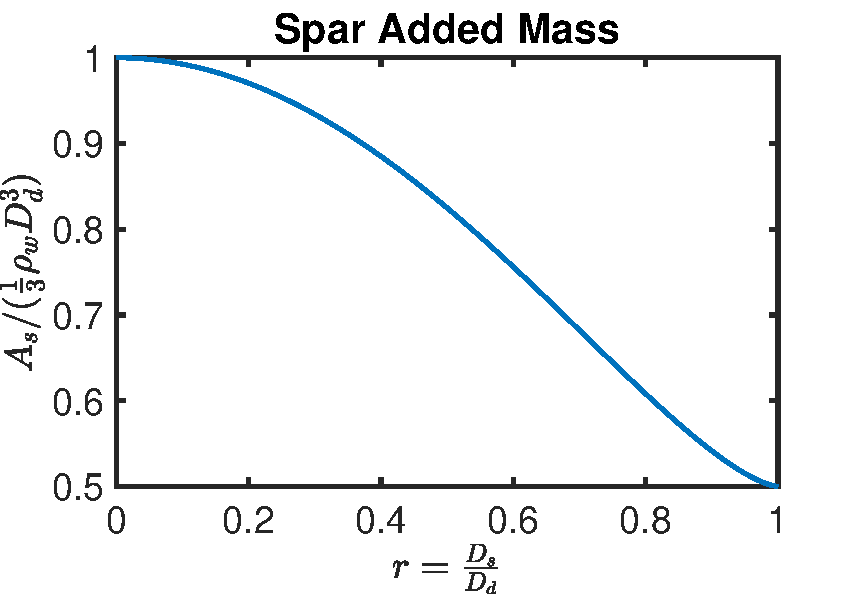
\includegraphics[width=0.5\linewidth]{figs/Figure_spar_added_mass.pdf}
    \caption{Nondimensional spar added mass as a function of column to damping plate diameter ratio}
    \label{fig:spar_added_mass}
\end{figure}
Meanwhile, the spar damping and excitation ($B_s$ and $\hat{\gamma}_s$) and the coupling damping and added mass ($B_c$ and $A_c$), are obtained by interpolating an existing WAMIT BEM solution for the nominal geometry.
Specifically, interpolation is performed over the nondimensional damping plate diameter $k D_d$.
For $|\hat{\gamma}_s|$, an additional multiplicative factor of $e^{-k (T_s - T_{s,nom})}$ is applied to account for the decrease of excitation with depth.

%  \paragraph{Spar Dynamics}
% The RM3 is a two-body system where the relative motion of the float and spar produces power. However, capturing these underactuated multibody dynamics would require more complicated modeling and control \cite{faedo_principle_2022}, especially in the context of force saturation%, as well as implementation of the excitation force phase in MEEM.
% While updating these models is important future work, a fixed spar is assumed for this study. Thus the results can be considered more dynamically representative of a single-body point absorber or a two-body point absorber with bottom-mounted spar, as might be encountered in shallow water. Nonetheless, calculations still utilize the 45 m water depth of Humboldt Bay, and the results provide relevant preliminary design insights about a floating spar device, especially because the spar structures and economics are still considered. To ensure that the fixed spar assumption is reasonably accurate, the spar amplitude is required to remain small.

% Rather than checking this requirement by calculating the spar amplitude exactly, as this would require the exact modeling complications which the fixed-spar assumption intends to circumvent, the characteristics of second-order linear systems are used to develop a simple sufficient criteria for low spar motion. The peak response amplitude of a system with equation of motion $m\ddot{x}+b\dot{x}+kx=F$ is:
% \begin{equation}
%     |X|_{pk} = \begin{cases}\frac{1}{2\zeta\sqrt{1-\zeta^2}} \frac{F}{m\omega_n^2} & 0<\zeta < 1\\
%     \frac{F}{m\omega_n^2} & \zeta \geq 1
%     \end{cases}
% \end{equation}
% where damping ratio is $\zeta=\frac{b}{2\sqrt{mk}}$ and natural frequency is $\omega_n=\sqrt{\frac{k}{m}}$. To keep the peak spar amplitude $|X|_{pk}$ low, both $\zeta$ and $m\omega_n^2/F=k/F$ should be kept high. A sufficient criteria for maintaining $|X|_{pk}$ below some nominal threshold $|X|_{pk,nom}$ is therefore to constrain $\zeta=\zeta_{nom}$ and $k/F > (k/F)_{nom}$. While this is not a necessary condition (other designs could also maintain low spar amplitude), a sufficient condition is adequate for preliminary optimization purposes. 

% Expressing these conditions in terms of the uncontrolled spar dynamic coefficients \cite{tao_low_2003}:
% \begin{equation}\label{eq:spar}
% \begin{aligned}
% b &= b_{s,rad}+b_{s,drag} \\
% k &= \frac{\pi}{4} \rho_w g  D_s^2 \\
% m &= \rho_w V_{sub,s}C_m\\
%     \omega_n^2 &= \frac{g}{C_m D_d} \frac{1}{\frac{T_s}{D_d} + \frac{h_d}{D_d}\left(\frac{D_d}{D_s}\right)^2} \leq \omega_{n,nom}^2 \\
%     \zeta &= abcd \geq \zeta_{nom}
% \end{aligned}
% \end{equation}
% where $C_m$ is the spar inertia coefficient.

% The geometry is required to maintain at least as high damping ratio and at least as low natural frequency as the nominal RM3 design. While this single-body spar analysis does not take into account the dynamic effect of the PTO force on the spar, it is sufficient to provide confidence that the spar response remains similar enough to the nominal design that the float can be analyzed assuming a fixed spar.

% \hl{Describe the frequency dependent fudge factor and add a figure showing that ratio as a function of sea state.} MDOcean scales the fixed-spar mechanical power by a period-dependent rational tuning factor 
% \begin{equation}
%     P_{spar~floating} = \frac{c_1}{c_2T^2+c_3T+c_4} P_{spar~fixed}
% \end{equation}
% which adjusts only the power (not the amplitude). A fit of MDOcean and RM3 report yielded $[c_1,c_2,c_3,c_4]=[23,1,-15,86]$, and the coefficients can be set to $[1,0,0,1]$ to disable the tuning. 

A second limitation of the present implementation of MEEM is numerical overflow.
To prevent overflow, each fluid region must exceed a minimum height $ \Delta z_{min}$ that is proportional to the region diameter $D$:
\begin{equation}\label{eq:delta-z-min-intro}
    \Delta z_{min} \sim D
\end{equation}
for both the spar ($\Delta z_s, D_s$) and the float ($\Delta z_f, D_f$), with variables shown in \figurename~\ref{fig:meem-geom}.
The constant of proportionality between $\Delta z_{min}$ and $D$ is discussed in \appendixname~\ref{sec:MEEM_details} and is sufficiently small that realistic geometries do not come close to numerical overflow. 

%The current implementation of MEEM yields only the magnitude, not phase, of the excitation coefficient (using equation 99 rather than 97 of \cite{chau_inertia_2012}). Therefore the phase is set to zero, an approximation that will be shown in the following section to be adequate for single body dynamics.

Figure \ref{fig:meem-hydro-coeffs} shows the hydrodynamic coefficients as a function of wave frequency $\omega$ for the nominal RM3 geometry. 
\begin{figure}
\centering
\includegraphics[width=\linewidth]{\matlabFilepath{6}}
\caption{Hydrodynamic coefficients vs. frequency}\label{fig:meem-hydro-coeffs}
\end{figure}
The MEEM results for the simplified cylindrical geometry are a close match to WAMIT BEM results for the exact RM3 geometry, except at frequencies below 0.3 rad/s.
This is expected because the BEM solution assumes infinite depth, which requires a finite added mass at low frequency, whereas MEEM uses finite depth, where the added mass must grow logarithmically toward infinity at zero frequency \cite{mciver_added_1991}.
For the site under consideration, the lowest-frequency sea state containing any energy is 0.4~rad/s, so the discrepancy is not a concern.

%TC:break Dynamics and Control
\subsubsection{Dynamics and Control}\label{sec:dynamics}
\paragraph{Modified Frequency Domain Techniques}
Methods for WEC dynamics and control simulation in an optimization context were reviewed in section~\ref{sec:lit} and include time-stepping (nonlinear, numerical, high computation cost), frequency domain (linear, analytical, low computation cost), pseudo-spectral (nonlinear, numerical, medium computation cost), modified frequency domain techniques (approximate nonlinear, semi-analytical, low computational cost), and Pontryagin's maximum principle (nonlinear, analytical, low computational cost).
MDOcean requires the ability to incorporate nonlinearities, at least approximately.
Inherent nonlinearities such as drag significantly affect the amplitude and power production at resonance.
Even with linearized intrinsic dynamics, maintaining optimality subject to dynamic constraints also requires a nonlinear controller.
Dynamic constraints on amplitude, force, and peak power significantly influence the trade-off of power and cost, and amplitude limits are required to obtain a physically meaningful result.
Besides nonlinearities, MDOcean also requires a low computation cost, since the dynamics will be evaluated many thousands of times during optimization.
Of the methods mentioned, Pontryagin's maximum principle (PMP) and modified frequency domain techniques meet these requirements.
PMP requires an analytically difficult derivation unique to the specific nonlinearities in question because wave energy dynamics have a particular form requiring so-called singular control \cite{zou_optimal_2017}.
On the other hand, modified frequency domain techniques are simple and intuitive.
Therefore, MDOcean pursues a quasi-linear semi-analytical modified frequency domain method.

When handling dynamic constraints with a modified frequency domain method, first the unconstrained optimal controller (and the response signals corresponding to that controller) are determined in the frequency domain.
If the response for a given sea state does not violate any constraints, then the unconstrained controller and corresponding power is used for that sea state.
Otherwise, a variety of approaches are possible to address the violated constraint, summarized in Table~\ref{tab:constraint-approaches} and described below. 

\begin{table}
\centering

\begin{tabular}{>{\raggedright\arraybackslash}p{0.6\linewidth}l l} 
\textbf{Approach} & \textbf{Accuracy} & \textbf{Optimality} \\ \hline
(1) Nonlinear optimal (or near-optimal) controller, linearized via describing functions& High & High \\
(2) Linear optimal controller& High & Medium \\
(3) Saturate or zero the
times with constraint violations, neglecting effect on response& Medium & Medium-low\\
(4) Saturate or zero entire sea state& Low & Low \\
(5) Mark design as infeasible& N/A& Lowest \\

\end{tabular}
\caption{Constraint Satisfaction Approaches for Modified Frequency Domain Methods}
    \label{tab:constraint-approaches}
\end{table}

The modified frequency-domain approach with the highest accuracy and optimality (1) is to synthesize a new nonlinear optimal (or near-optimal) time-domain controller that obeys the constraint, taking into account the linearized effect of that nonlinear controller on the frequency domain response.
If a time-domain PMP control law is available for the constraint under consideration, it can be used as the nonlinear optimal controller directly.
This differs from the standard PMP method in that the response and power corresponding to the time-domain PMP controller is determined in the frequency domain, rather than via numerical time-integration (as in \cite{zou_optimal_2017}) or analytical time-integration (as in \cite{lin_fast_2025}).
For situations without an explicit PMP control law, a nonlinear near-optimal controller can be constructed using insights from signal saturation and filtering, which is the approach pursued here for the force limit.
In either case, the nonlinear controller is linearized via the describing function method.

If a nonlinear controller or the corresponding describing function to linearize it are not available, the most optimal linear controller that obeys the constraint can be used instead (2).
This requires some frequency-domain calculations for an impedance-mismatched linear system described in \cite{mccabe_force-limited_2024} and can be visualized with the Smith chart, a tool common in electrical engineering.
This approach accurately reflects the maximum power that a linear controller could produce, although this power will be lower (less optimal) than that of the optimal nonlinear controller. 

If the implementation for the optimal constrained linear controller is also not available, then the violating portion of the time-domain signals can be saturated or zeroed (3).
This approach neglects the corresponding effect of the saturation/zeroing on other quantities in the system, which lowers the accuracy, and the controller does not have the opportunity to even approximately consider the constraint, resulting in a power production potentially much lower than the constrained optimal.
This simple approach does not require any derivations to implement.
It has been used in several previous WEC optimization studies for various constraints \cite{garcia-teruel_design_2022,garcia-teruel_reliability-based_2021,cotten_multi-objective_2022,mccabe_constrained_2013} and is evidently the most common modified frequency domain method in the marine energy field.
It is utilized here for the power limit.

As a last resort, the energy in that sea state can be zeroed (4), essentially assuming that the device enters survival mode in those cases to avoid constraint violation, or the entire design can be marked infeasible with a constraint in the optimization (5), which \cite{mccabe_constrained_2013} pursues for a radiation limit constraint.
These approaches do not attempt to find dynamic solutions which satisfy the limits, and essentially deal with violations by penalizing the optimization though either the objective or constraints.
The latter approach (5) is actually the only option for slamming amplitude limits in the storm design load case, since the device is already in survival mode and not producing power or applying a control input.
Approach (5) is also pursued here for amplitude limits in the operational design load case, in the interest of consistency and expedience. 

In future work, MDOcean could instead utilize describing functions (1) and the optimal constrained linear controller (2) for the power and operational amplitude limits respectively to improve accuracy and optimality.
The describing function for force saturation is prioritized due to its simpler implementation as well as the force constraint's frequent activity and strong impact on results observed in prior RM3 optimizations \cite{mccabe_multidisciplinary_2022,gaebele_tpl_2025,mcgilton_optimal_2024}.
A describing function (1) is also utilized for the drag nonlinearity.
Table~\ref{tab:nonlinearities} summarizes the dynamic nonlinearities and limits and the method MDOcean currently uses to handle each.

\begin{table}
    \centering
    \begin{tabular}{>{\raggedright\arraybackslash}p{0.25\linewidth}>{\raggedright\arraybackslash}p{0.7\linewidth}}
         \textbf{Dynamic nonlinearity/limit}& \parbox{\linewidth}{\centering\textbf{Method}}\\ \hline
         Drag& Describing function (1) for $\sin(\omega t)|\sin(\omega t)|$ with iteration to find effect on response and optimal controller\\
         Force limit& Describing function (1) for $\text{sat}(\sin(\omega t))$ with iteration to find effect on response and optimal controller\\
         Power limit& Average value of $\text{sat}(\sin(\omega t)+C)$, neglecting any effect on response and optimal controller (3)\\
  Amplitude limit&Optimizer considers limit violations as infeasible designs (5)\\\end{tabular}
    \caption{Dynamic nonlinearities and approach for each}
    \label{tab:nonlinearities}
\end{table}

Describing functions assume a certain time-domain nonlinear signal shape and then calculate the fundamental amplitude of that signal for use in a typical frequency-domain simulation.
For a force signal, the fundamental amplitude is most the relevant harmonic because not only is it typically the largest amplitude, but it undergoes the least amount of filtering by the low-pass plant and therefore contributes the most to power production.
Because the fundamental amplitude depends on the response, the frequency domain simulation is only quasi-linear and must either be iterated numerically or solved analytically.
MDOcean uses iteration to handle both the drag and saturation nonlinearity. % and an analytical solution for the force saturation nonlinearity.

While the describing function method used here has been known for over half a century, MDOcean represents its first application in a wave energy optimization or open-source simulation, to the authors' knowledge.
The RAFT open-source Python package for offshore wind turbines uses the drag describing function with iteration but does not include describing functions for saturation \cite{hall_open-source_2022}.
Thus, MDOcean's semi-analytical dynamics offer a combination of speed, accuracy, and simplicity that is novel in the wave energy space.

\paragraph{Equation of Motion}
The float and spar are each modeled as a floating rigid body, and the two bodies are coupled to transmit force between them.
\hl{Note to scrutineers: the typeset equation below is for a single rigid body (stationary spar), but the actual simulation uses the real two-body dynamics.
The two-body matrix equation will be typeset before submission.} The MDOcean dynamic model assumes %a stationary spar and
regular waves for reasons to be detailed later this section, so the system experiences monochromatic forced oscillation.
The equation of motion can be expressed in the time domain as: % todo: this is time domain so gamma is not allowed to be complex
\setlength\arraycolsep{0pt}
\newcolumntype{C}{>{{}}c<{{}}}
\begin{equation}\label{eq:eom}
\begin{array}{rCCCCC}
     m\ddot{x}(t) = & \underbrace{F_{e}(t)}_{\substack{\textrm{wave} \\  \textrm{excitation} }} & +\underbrace{F_{rad}(t)}_{\substack{\text{hydrodynamic} \\ \text{radiation} }} +&  \underbrace{ F_{res}(t)}_{\substack{\textrm{hydrostatic} \\ \text{restoring} }} &  +~~~~\underbrace{F_{d}(t)}_{\substack{\textrm{drag} }}~~~~+ & \underbrace{F_{p}(t)}_{\substack{\textrm{power}\\\text{takeoff} }} \\
    = & \overbrace{\hat{\gamma}~ \zeta(t)} & \overbrace{-A_h\ddot{x}(t) - B_h\dot{x}(t)} &  \overbrace{-K_hx(t)} & \overbrace{-B_d\dot{x}(t)-K_dx(t)}  & \overbrace{-B_p\dot{x}(t)-K_px(t)}
\end{array}
\end{equation}
where $x(t)$ (body position) and $\zeta(t)$ (wave elevation) were defined in section~\ref{sec:meem}.
Forces include wave excitation, hydrodynamic radiation, hydrostatic restoring, drag, and power takeoff.
For each force component, a linear or quasi-linear model is adopted, with coefficients $\vec{\hat{\gamma}}$, $\mathbf{A_h}$, $\mathbf{B_h}$, $\mathbf{K_h}$ from the hydrodynamics module and $\mathbf{B_d}$, $\mathbf{K_d}$, $\mathbf{B_p}$, and $\mathbf{K_p}$ to be derived in the following sections.
The excitation coefficient $\hat{\gamma}$ is complex, and all other coefficients are real.
In the frequency domain, the complex transfer function from real regular wave height $H$ to complex body amplitude $\hat{X}$ is then:
\begin{equation}\label{eq:eom-freq-domain}
    \frac{\hat{X}}{H} = \frac{\hat{\gamma}/2}{(m+A_h)s^2+(B_h+B_d+B_p)s+(K_h+K_d+K_p)}
\end{equation}
where $s=i\omega$ is the Laplace variable.

\paragraph{PTO Dynamics and Power Production}
A PTO model must capture the dynamics of any elements that transmit, transduce, or condition power between the rigid-body mechanical energy of the float and the end energy product, in this case electricity.
Relevant dynamics include the inertia, stiffness, static friction, mechanical advantage, losses, and electromagnetic coupling of flywheels, shafts, springs, gears, hydraulic circuits, generators, and power electronics.
Reference \cite{penalba_review_2016} reviews common WEC PTO models and \cite{coe_co-design_2024} synthesizes these into a multiport impedance matching network framework to facilitate control co-design.
Reference \cite{coe_co-design_2024} uses the transmission matrix form, which groups the effort and flow variables $e$ and $q$ at each port. 

A linear model of the drivetrain with mechanical transmission matrix $[a]_m$ takes the form
% impedance
% \begin{equation}
% \begin{bmatrix}
% F_p \\ \tau
% \end{bmatrix}
% =
% \underbrace{\begin{bmatrix}
% Z_{m,11} & Z_{m,12} \\
% Z_{m,21} & Z_{m,22}
% \end{bmatrix}}
% _{Z_m}
% \begin{bmatrix}
% \dot{X} \\ \Omega
% \end{bmatrix}
% \end{equation}
\begin{equation}
\begin{bmatrix}
F_p \\ \dot{X}
\end{bmatrix}
=
\underbrace{\begin{bmatrix}
a_{m,11} & a_{m,12} \\
a_{m,21} & a_{m,22}
\end{bmatrix}}
_{[a]_m}
\begin{bmatrix}
 \tau\\ \Omega
\end{bmatrix}
\end{equation}
where the PTO force $F_p$ and WEC velocity $\dot{X}$ are found as a function of the generator torque and rotation speed $\tau$ and $\Omega$.
Meanwhile, linear generator electrical dynamics are expressed with electrical transmission matrix $[a]_e$:
\begin{equation}
\begin{bmatrix}
 \tau\\ \Omega
\end{bmatrix}
=
\underbrace{\begin{bmatrix}
a_{e,11} & a_{e,12} \\
a_{e,21} & a_{e,22}
\end{bmatrix}}
_{[a]_e}
\begin{bmatrix}
 V \\ I
\end{bmatrix}
\end{equation}
with park-transformed quadrature electrical voltage and current $V$ and $I$.
The system operating point is determined by the controller, which is typically formulated at the generator mechanical port.
A linear control law with impedance $\hat{Z}_u$ split into damping and stiffness coefficients $B_u$ and $K_u$ has the form 
\begin{equation}
\tau = \hat{Z}_u \Omega =\left(B_u + \frac{K_u}{s} \right) \Omega
\end{equation}
The time-domain power $P(t)$ at any port is simply the product of the port effort and flow variables.
To facilitate this calculation in transmission form, power can be found as the quadratic product of the port variable vector with the two-dimensional exchange matrix $E_2$,
\begin{equation}
P(t) = e~q
= \frac{1}{2}
\begin{bmatrix}
 e \\ q
\end{bmatrix}^T
\underbrace{\begin{bmatrix}
0~ & 1 \\
1~ & 0
\end{bmatrix}}
_{E_2}
\begin{bmatrix}
 e \\ q
\end{bmatrix}
\end{equation}
where substituting $[e,q]^T=[F_p,\dot{X}]^T$ yields the floating body mechanical power, $[e,q]^T=[\tau,\Omega]^T$ yields the generator mechanical power, and $[e,q]^T=[V,I]^T$ yields the generator electrical power. 

Moving back to the frequency domain and assuming sinusoidal waveforms, the average and peak powers $P_{avg}$ and $P_{pk}$ in a given sea state can be found as:
\begin{equation}
\begin{aligned}
     P_{avg} &= \frac{1}{2}\Re(\hat{e} \hat{q}^*) = \frac{1}{2} \Re(\hat{Z})|\hat{q}|^2 
    \\
    P_{pk} &=  P_{avg} + \frac{1}{2}|\hat{e} \hat{q}^*| = P_{avg}\left( 1 + \sqrt{1 + \left(\frac{\Im(\hat{Z})}{\Re(\hat{Z})}\right) ^2  } \right)
\end{aligned}
\end{equation}
if the port is terminated with complex impedance $\hat{Z}$. 

Rather than utilize detailed PTO models for co-design, which a number of recent papers (e.g. \cite{coe_useful_2023,gaebele_incorporating_2023} and those discussed in section \ref{sec:lit}) have already proven the value of, this study chooses to keep the PTO design unspecified by assuming a constant-gain, infinite bandwidth transmission system and a generator with fixed average efficiency $\eta$.
While obviously unrealistic and insufficient for designing the device's actual PTO hardware, this decision adds simplicity and illustrative value at the system level.
It highlights the effect of the novel non-PTO (e.g. structural) aspects of WEC co-design that this study introduces while still capturing the effect of PTO rating on system performance and maintaining sufficient generality to incorporate more detailed PTO models in the future.
Furthermore, setting $\eta=80\%$ maintains consistency with the RM3 design assumption of \cite{RM3} to facilitate comparison and validation. 

More specifically, rather than implement a full generator electrical transmission matrix $[a]_e$, for the optimization study a simple average efficiency $\eta$ describes the gain between the average mechanical power and average electrical power.
This is not necessarily equivalent to an assumption that the generator itself has constant efficiency, since controllers with reactive terms ($K_u\neq 0$) spend some time expending energy, which reverses the direction of the generator efficiency.
The average efficiency is assumed to also apply to the peak powers, though this is not guaranteed in general for the same reason.
\begin{equation}\label{eq:power-elec}
\begin{bmatrix}
P_{avg,elec} \\
P_{pk,elec}
\end{bmatrix}
= 
\eta
\begin{bmatrix}
P_{avg,mech} \\
P_{pk,mech}
\end{bmatrix}
= 
\eta \frac{1}{2} B_u |\hat{\Omega}|^2
\begin{bmatrix}
1 \\
 1 + \sqrt{1 + \left(\frac{K_u}{B_u \omega }\right) ^2  }
\end{bmatrix}
\end{equation}
Additionally, the drivetrain mechanical transmission matrix $[a]_m$ is set to the identity matrix, which represents a static effective gear radius $R=1$:
\begin{equation}
[a]_m = \begin{bmatrix}
1/R &~ 0 \\
0 &~ R
\end{bmatrix} = \begin{bmatrix}
1 &~ 0 \\
0 &~ 1
\end{bmatrix}
\end{equation}
With this $[a]_m$, the control damping and stiffness $B_u$ and $K_u$ equal the PTO damping and stiffness $B_p$ and $K_p$.
This will simplify the impedance matching procedure described below, requiring matching at only one interface.

%The time-domain mechanical power is $P_{mech}(t) = \tau(t) \Omega(t) = (B_u \Omega(t) + K_u \theta(t) ) \Omega(t) $, where $\theta(t)$ is the generator rotational position. Assuming sinusoidal waveforms, the time-average and peak mechanical power in a given sea state are then

\paragraph{Force-Constrained Optimal Reactive Control}
In the absence of constraints, maximizing absorbed power requires impedance matching.
At the mechanical interface between the floating body and PTO, this means that the force of the PTO on the WEC, described by $F_{p} = B_{p}\dot{X} + K_{p}X$, must have an impedance that is the complex conjugate of the WEC's intrinsic impedance.
This is called reactive control, with subscript $reac$:
\begin{equation}\label{eq:matched-controller}
	B_{p,reac} = B_h + B_d, \qquad K_{p,reac} = (m+A_h) \omega^2 - K_h - K_d
\end{equation}
However, the nominal RM3 design features a hydraulic system which lacks reactive capability (the ability to function as a motor and add energy to the system at some times).
Avoiding reactive power restricts the system to so-called damping control, with subscript $damp$, and requires $K_{p,damp}=0$.
The power-maximizing PTO damping $B_{p,damp}$ is then
\begin{equation}\label{eq:damping-control}
    B_{p,damp} = \sqrt{ (B_{p,reac})^2 + (K_{p,reac}/\omega)^2}
\end{equation}

Both of these controllers frequently result in excessively large generator torques, especially in reactive control when $K_u=K_p$ is far from zero. $K_{p,reac}$ is often a large negative number because cost minimization favors a low mass, and the negative PTO damping reduces the natural frequency to better match the ocean wave frequency with a smaller device mass.
Control laws \eqref{eq:matched-controller} and \eqref{eq:damping-control} provide no mechanism to reduce this torque.
Actuator torque limits are important to model.
Leaving the generator torque unbounded when modeling energetic sea states would result in excessive structural and powertrain requirements.
In response, two strategies are pursued at once: (1) to create an intentional linear impedance mismatch, sacrificing power to satisfy a torque limit, and (2) to use nonlinear control to enable satisfaction of the torque limit with less of a power sacrifice.

Actuator limits change the optimal force signal from a pure sinusoid to a saturated waveform, approaching a square wave for sufficiently low force limit.
As is, this nonlinear signal could not be handled with a frequency-domain transfer function and would require time-domain simulation.
Conveniently, through the describing function method, the saturated signal can be represented with Fourier analysis as a superposition of harmonics.
Furthermore, because the plant is a second order oscillator and filters out high frequency inputs, harmonics other than the fundamental contain very little energy and can be safely neglected.
Figure \ref{fig:sat} shows this approximation graphically for a saturated-sine force signal.
\begin{figure}
\centering
\includegraphics[width=.7\linewidth]{\matlabFilepath{7}}
\caption{Saturated sin vs. time (red) and its fundamental amplitude (blue)}\label{fig:sat}
\end{figure}
Details of the calculation are provided in \appendixname~\ref{sec:appendix-force-sat}.
The result is updated values for control gains $B_u$ and $K_u$ that result in a torque that obeys the force constraint and is used in place of equations~\eqref{eq:matched-controller} and \eqref{eq:damping-control}.

\paragraph{Drag}
Modeling drag force is important to avoid unrealistically high resonant peaks in the response amplitude and the resulting overestimate in power production.
Drag force $F_d$ is proportional to the product of the relative velocity of the WEC and wave, $\dot{x}_{rel}(t)=\dot{x}(t)-\dot{x}_{wave}(t)$, with its absolute value.
The use of the relative velocity rather than direct WEC velocity means that the drag contributes not only a damping-like effect, described with coefficient $B_d$, but also a small stiffness-like effect, with coefficient $K_d$.
The quadratic form $|F_d|\sim|\dot{x}_{rel}|^2$ implies a nonlinear input-output response that would normally require time-domain simulation.
To improve computational efficiency and allow solution in the frequency domain, the nonlinearity is quasi-linearized with another describing function, following \cite{quartier_influence_2021}:
\begin{equation}
\begin{aligned}
    F_{d}(t) &= \frac{1}{2}\rho_w C_d A_w ~\dot{x}_{rel}(t) |\dot{x}_{rel}(t)| \\     
    &= \frac{1}{2}\rho_w C_d A_w ~\dot{X}_{rel}^2 \sin(\omega t) | \sin(\omega t)|\\
    &\approx \frac{1}{2}\rho_w C_d A_w ~\dot{X}_{rel}^2\frac{8}{3\pi} \sin(\omega t)\\
   % F_{d}(\omega)&= \frac{1}{2}\rho_w C_d A_w \frac{1}{2\pi}\dot{X}_{rel}(\omega)*|\dot{X}_{rel}(\omega)| \\
    %\approx  \frac{1}{2}\rho_w C_d A_w \frac{8}{3\pi}  \dot{X}_{rel,1}(\omega)\dot{X}_{rel,1}(\omega) \\
    &= B_{d} \dot{X} + K_{d} X
    \end{aligned}
\end{equation}
with drag coefficient $C_d$.
The nonlinear waveform and describing function approximation are compared in Figure~\ref{fig:drag-df}.
The amplitude of the sinusoidal approximation equals $\frac{8}{3\pi}\approx0.85$ times the peak of the nonlinear waveform.
\begin{figure}
    \centering
    \includegraphics[width=.7\linewidth]{\matlabFilepath{8}}
    \caption{Conceptual demonstration of the drag describing function in the time domain.
The nonlinear signal (red) is approximated by its fundamental amplitude (blue).}
    \label{fig:drag-df}
\end{figure}

The resulting magnitude and phase of WEC motion are obtained by numerically iterating the state-dependent coefficients $B_{d}$ and $K_{d}$.
Further derivation, convergence details, and control implications are discussed in \appendixname~\ref{sec:appendix-drag}.

%\paragraph{Power Saturation}
%Equation~\eqref{eq:mech-power} shows that the power peak to maximum ratio is at minimum two for a damping controller, 
%\hl{describe}

\paragraph{Energy Production}
To find the overall average power production $P_{avg,elec}$ in a location with a given distribution of sea states, $P_{avg,elec}(H,\omega)$ for each sea state is weighted by that sea state's probability using a Joint Probability Density (JPD) matrix.
This method is illustrated in Figure \ref{fig:JPD-muptiply}.
The JPD used in this analysis represents wave conditions in Humboldt Bay, CA and is taken from reference \cite{noauthor_system_2020}.

\begin{figure}
\centering
\includegraphics[width=\linewidth]{\matlabFilepath{9}}
\caption{Power matrices multiplication}
\end{figure}\label{fig:JPD-muptiply}

%As expected, low-frequency sea states achieve mechanical powers close to the radiation limit (device capture efficiencies near one), and high frequency sea states achieve mechanical powers equal to the amplitude limit.

The annual energy production $AEP$ in kWh/year is the product of the number of devices, the average power per device, an efficiency $\eta_{array}$ representing transmission losses and array downtime, and an appropriate constant to convert from Watts to kWh/year:
\begin{equation}
    AEP = N_{WEC} ~ P_{avg,elec} ~\eta_{array} \frac{8766}{1000}
\end{equation}

%Finally, the standard deviation $\sigma$ of power across all sea states $P(\omega)$ is computed, and normalized by the average power $\mu$ to get the coefficient of variation (see equation \eqref{cv}).

\paragraph{Dynamic Limits and Design Load Cases}
This study considers two design load cases: (1) cyclic operational loading in sea states where power is produced, and (2) storm loading in sea states where the device enters survival mode and stops producing power.
These correspond roughly with the 1-year and 50-year return periods specified in the wave energy design standard IEC TS 62600-2, and with the fatigue limit state (FLS) and ultimate limit state (ULS) in offshore wind standards.
When the WEC is in survival mode, an external brake locks the PTO, enforcing the float and spar to move together without loading the generator.
This section details the maximum amplitudes and forces in each case.
Currently all sea states in the JPD with nonzero probability are considered operational, since the generator force and power limit serve to reduce loads in energetic sea states.
Future studies could control the transition from operational to survival mode more finely, perhaps with an additional design variable representing an operational incident energy threshold.

The heave forces in equation \eqref{eq:eom} can be separated into fluid forces, which act on the vertically-oriented wetted surface of the body, the inertial force, which for dynamic purposes is assumed to act at the center of mass but for structural purposes actually acts distributed over the material, and the PTO force, which acts at the connection between the float and the spar.
The vertical design load $F_{heave}$ is taken as the maximum of the PTO and fluid force amplitudes, which conservatively neglects the spatial distribution of the D'Alembert forces:
\begin{equation}
\begin{aligned}
    F_{heave,f} &=\max(|F_p|, |m_f\ddot{X}_f-F_p|) \\
    F_{heave,s} &=\max(|F_p|, |m_s\ddot{X}_s-F_p|)
\end{aligned}
\end{equation}
where table~\ref{tab:DLCs} details $F_p$ and $X$ based on the assumptions of each design load case.

\begin{table}
    \centering
    \begin{tabular}{>{\centering\arraybackslash}p{0.3\linewidth}>{\centering\arraybackslash}p{0.3\linewidth}>{\centering\arraybackslash}p{0.3\linewidth}}
 & \multicolumn{2}{c}{\textbf{Design Loadcase}}\\\cline{2-3}
         \textbf{Variable}& \textbf{1: Operational}&\textbf{2: Storm}\\ \hline
         Powertrain force, $F_p$& \parbox[m]{\linewidth}{\centering Force provided by generator so saturates at $F_{max}$} & \parbox[m]{\linewidth}{\centering Force provided by brake, so no saturation.
Solve \eqref{eq:eom-freq-domain} for $F_p$.}\\ 
 Float amplitude, $X_f$& \parbox[m]{\linewidth}{\centering Given by \eqref{eq:eom-freq-domain} (2-DOF)}& \parbox[m]{\linewidth}{\centering Given by \eqref{eq:eom-freq-domain} (1-DOF) with $F_p=0$}\\ 
         Spar amplitude, $X_s$& Given by \eqref{eq:eom-freq-domain}&Equals $X_f$ due to brake\\
 \parbox[m]{\linewidth}{\centering Maximum allowable relative amplitude between float and spar, $|X_f-X_s|_{max}$ \vspace{8pt}}& \shortstack{$\min(h_{fs,clear},h_{fs,up},$\\$h_{fs,down})$} &N/A\\
 \parbox[m]{\linewidth}{\centering Maximum allowable float amplitude, $|X_f|_{max}$ }& $\min(X_{f,linear}, X_{f,slam})$& N/A \\ %$X_{slam}$\\
 \parbox[m]{\linewidth}{\centering Maximum allowable spar amplitude, $|X_s|_{max}$ }& $\min(X_{s,linear}, X_{s,slam})$& N/A %$X_{slam}$\\
    \end{tabular}
    \caption{Force components in each design load case}
    \label{tab:DLCs}
\end{table}

The calculation of forces and amplitudes in operational seas uses the 2-DOF equation of motion \eqref{eq:eom-freq-domain} with the PTO force $F_p$ set by the chosen controller.
In storm seas, the brake force could calculated by solving the 2-DOF equation of motion for the force necessary to enforce zero relative motion between the float and spar.
%However, it is not actually necessary to calculate the brake force, since the PTO cost model does not contain a term for the brake cost. -- this is not true, even without a PTO cost model, the brake force is needed to calculate the heave force for structural purposes.
However, this would require additional time-consuming iteration.
Therefore, instead of separately finding the float and spar heave force, the net heave force on both bodies is calculated using the 1-DOF equation of motion \eqref{eq:eom-freq-domain} with zero PTO force $F_p=0$ (since the brake force is an internal force when considering a unifed float-spar rigid body) and the hydrodynamic coefficents corresponding to the float only.
\hl{(Note: ideally it would use hydro coefficients for the merged float-spar geometry, subscript m in the hydro module).}
For conservativism, this net force is assumed to apply to both the float and spar independently. % For force, this makes way less sense than doing the 2-DOF calc, since the net float-spar force isn't what matters for structures. For amplitude, this is a fine assumption, but I'm not even using the storm amplitude constraint, so it doesn't make any sense.

Meanwhile, the surge force for each component is calculated as \cite{newman_motions_1963}
\begin{equation}\label{eq:surge-force}
   F_{surge} = \frac{H\rho_w \omega^2 A_w}{k} (e^{-kz_{top}}-e^{-kT})
\end{equation}
using the respective waterplane areas $A_w$  and drafts $T$ for the float and spar.
The top vertical height $z_{top}$ is set to zero for the float and $T_{f,2}$ for the spar.
The design surge force is the maximum surge force over all nonzero-probability sea states.
Equation~\eqref{eq:surge-force} assumes a slender cylinder with diameter much smaller than the wavelength and may be less accurate for the float due to diffraction effects.
Incorporating semi-analytical hydrodynamic coefficients for surge is a possible area of future work. 
Maximum acceptable heave %and surge 
forces will be evaluated with structural factors of safety in \ref{sec:structures}.
The structures model currently lacks the ability to account for surge forces, so the surge force calculation is not used in the optimization.

The table also indicates the maximum permissible amplitudes.
In operational sea states, the geometric clearance between the float and spar is enforced to prevent overtravel.
The permissible heights for upward and downward motion of the float relative to the spar are:
\begin{equation}\label{eq:h-fs-up-down}
    h_{fs,up} = h_s - T_s - (h_f- T_{f,2}), \qquad h_{fs,down} = T_s - T_{f,2} - h_d
\end{equation}
Additionally, a limit of $h_{fs,clear}$ (see definition in \figureautorefname~\ref{fig:dims}) is required to ensure clearance of the tubular structure connecting the float and spar.

Meanwhile, the conditions for linear wave-body interaction are enforced to maintain compatibility with the linear potential flow theory approach of \ref{sec:meem}.
This maximum amplitude $X_{linear}$ for the float and spar respectively is:
\begin{equation}
    X_{f,linear} = D_f/10, \qquad X_{s,linear}  =D_s/10
\end{equation}

In both operational and storm states, slamming should be avoided since it causes extremely high loads.
Slamming refers to the bottom surface of the WEC rising out of the water and hitting the free surface as it reenters (bottom-slamming), or symetrically the top of the WEC becoming fully submerged beneath the free surface (top-slamming).
The formula for the critical slamming amplitude $X_{slam}$ in regular waves of height $H$ is derived in \appendixname~\ref{sec:appendix-slam} and shown to lie between $\Delta z-H/2$ and $\Delta z+H/2$ for relevant vertcal body dimenson $\Delta z$, depending on the wave parameters and body diameter and oscillation phase.
For operational waves, $\Delta z$ for float bottom-slamming is taken as $T_{f,1}$ rather than $T_{f,2}$ since in addition to preventing slamming on the slanted surface of the float, this maintains constant waterplane area and thereby avoids unmodeled nonlinearities in the hydrostatic stiffness and Froude-Krylov excitation force.
Likewise for spar bottom-slamming, setting $\Delta z$ to $T_s-h_d$ not only avoids slamming on the bottom of the spar but also prevents the damping plate from surfacing.
The relevant $\Delta z$ for float and spar top-slamming in operational waves are the above-water heights $h_f-T_{f,2}$ and $h_s-T_s$ respectively.
For storm waves, currently the slamming limit is not applied.
%since calculation of the amplitude requires hydrodynamic coefficents for the float and spar acting as a single merged body, which the hydrodynamics module does not currently calculate. 
In future work, the storm $\Delta z$ should be set to $T_{f,2}$ to avoid slamming only on the bottom surface of the float.

Note that the analysis of this section continues to use standard linear wave theory with equivalent regular waves, even for the storm condition.
This is a questionable assumption, but it is necessary because optimization-suitable models for nonlinear wave forces do not currently exist.
Section~\ref{sec:discussion} will discuss possible future alternatives to this modeling choice.

% Todo: This table \ref{tab:sea-state} is \hl{possibly out of date now:}
% \begin{table}
% \centering

% \begin{tabular}{| l  |>{\raggedright\arraybackslash}p{0.35\linewidth}|>{\raggedright\arraybackslash}p{0.35\linewidth}|}
% \hline
% \textbf{Value} & \textbf{Sea state to use} & \textbf{Saturation to meet it?} \\
% \hline
% $F_{heave,storm}$& Storm sea state & Not relevant (controller is off during storm) \\
% \hline
% $F_{heave,op}$& Operating sea states with nonzero JPD & Ideally, but requires more work \\
% \hline
% $F_{pto}$& Operating sea states with nonzero JPD & Analytical \\
% \hline
% $X_{linear}$& Operating sea states with nonzero JPD & Ideally, but requires more work \\
% \hline
% $X_{slam}$& Storm sea state & Not relevant (controller is off during storm) \\ \hline 
%  $X_{fs}$& Operating sea states with nonzero JPD&Ideally, but requires more work\\\hline
% $P_{max}$& Operating sea states with nonzero JPD & Ideally, but requires more work \\
% \hline

% \end{tabular}
% \caption{Sea states}
% \label{tab:sea-state}
% \end{table}

\paragraph{Irregular Waves}
MDOcean uses a JPD to capture the long-term variation in wave conditions and accurately estimate annual average power and fatigue load.
Additionally, it assumes that each wave condition within the JPD is a sinusoidal regular wave.
Regular wave height $H$ and period $T$ are selected to provide equal energy as the irregular sea state:
\begin{equation}
    H = \frac{H_s}{\sqrt{2}}, \qquad T = T_e \approx 0.857 ~T_p 
\end{equation}
where the irregular sea state has significant wave height $H_s$, energy period $T_e$, and (for a Pierson-Moskowitz spectrum) peak period $T_p$.
This regular wave assumption avoids the time-consuming convolution integral or state-space identification that is typically required to simulate nonlinear dynamics subject to irregular wave forcing.

In the absence of dynamic constraints, the regular wave assumption does not significantly affect power production if the ultimate design utilizes a high-order linear controller capable of impedance matching over the bandwidth of each sea state.
If the ultimate design instead utilizes a simple PI controller, the assumption slightly overestimates the power produced in a broadband wave environment.
A previous study using a Bretschneider spectrum found the power generation for a point absorber with PI control to be around 92\% of the perfectly matched power \cite{coe_practical_2021}, which is sufficiently close to justify the approximation for early design phases without worrying about the complexity tradeoff of controller order.
Nonetheless, irregular time-domain transient peaks and the variation of hydrodynamic coefficients over the spectral width of each individual sea state are not considered.
Therefore, MDOcean likely underestimates the sensitivity to peak force, power, and amplitude constraints.
Section~\ref{sec:discussion} will discuss possible future extensions to incorporate irregular wave effects into the analysis.

\paragraph{Validation of Dynamics using WEC-Sim}
The popular time-domain hydrodynamic simulation software WEC-Sim \cite{ruehl_wec-simwec-sim_2024} is used to validate the dynamics module.
The WEC-Sim RM3 example is run with regular waves and with the device constrained to oscillate only in heave.
Notably, the RM3 geometry provided in WEC-Sim differs slightly from the published dimensions in the RM3 report, so for validation the dimensions input to MDOcean are adjusted to match WEC-Sim.

%Both fixed-spar and floating spar configurations are tested to understand the implications of MDOcean's fixed-spar assumption.
WEC-Sim runs utilize hydrodynamic coefficients obtained with the WAMIT BEM for dynamics, and control coefficients calculated with MDOcean for consistency.
MDOcean is run with MEEM as usual, and separately also run with the WAMIT coefficients % and with a modified version of the WAMIT coefficients with zero excitation phase.
to distinguish differences caused by disparate hydrodynamic coefficients from those caused by the underlying dynamics. 

The error in average power compared to the WEC-Sim power is less than 0.1\% in the best case and 38.2\% in the worst case, with an error breakdown for all simulation scenarios and sea states shown in Figure~\ref{fig:error-histogram}. 

\begin{figure}
    \centering
    \includegraphics[width=1\linewidth]{\matlabFilepath{10}}
    \caption{Error breakdown based on WEC-Sim Validation Runs}
    \label{fig:error-histogram}
\end{figure}
% Results reveal that the assumption of zero excitation phase ($\gamma=|\gamma|$) has no effect for single body dynamics in the absence of drag, extremely minor effect (0.34\% annual energy) for fixed-spar dynamics in the presence of drag, and major effects for floating-spar dynamics. 

Results reveal that the drag describing function and MEEM hydrodynamic coefficients have a minor effect assuming a 1-DOF system (9.7\% and 2.7\% error on the average power and maximum amplitude respectively) but a major effect on the 2-DOF system (38.2\% and 28.6\% respectively).
The extremely low errors in the 2-DOF system enforcing the same hydrodynamic coefficients as WEC-Sim and with zero drag (0.2\% and 1.9\% in power and amplitude respectively) indicate that this is not an error in the 2-DOF dynamic model itself, but in the way that a 2-DOF model amplifies errors in drag and hydrodynamic coefficients due to the importance of the phase of motion between each DOF. 
These errors are deemeed acceptable for the purposes of this study, since the goal is to demonstrate the value of simultaneously optimizing multiple disciplines and the ability to quickly evaluate a large number of design options.
More details on the WEC-Sim validation are described in \appendixname~\ref{sec:appendix-wecsim}.

%TC:break Structures
\subsubsection{Structures}\label{sec:structures}
The MDOcean structures module uses forces from the dynamics module as well as area and volume outputs from the geometry module to calculate the factors of safety for various structural failure modes.
The factors of safety represent the multiplicative increase in force before stress would surpass peak limits for storm loads and the endurance limit under operational loads.
Again aligning with the modeling philosophy of investing the up-front development time to create a simulation that runs extremely quickly with moderate accuracy, MDOcean integrates a combination of explicit algebraic and tabulated semi-analytical structural models that are well-established in the structures community yet rarely utilized for WEC design.
The structures module therefore runs significantly faster than traditional finite element method (FEM) simulations, though it lacks the ability to easily generalize to other geometries, boundary conditions, and load cases as a FEM model could. 

More specifically, the peak limits analyzed include yield, global buckling, local buckling, and ultimate where appropriate, while the endurance limit assesses high-cycle fatigue.
The latter is potentially conservative, and future work could implement Miner's law to better represent infrequent operational loads (low-cycle fatigue) \cite{ove_arup__partners_ltd_structural_2016}. 

The factor of safety is directly calculated for the most heavily loaded subcomponent in each of the three components: the bottom plate in the float, the cylindrical shell of the spar, and the annular plate of the damping plate.
Thicknesses of other subcomponents are either held constant or scaled with the dimensions of subcomponents that are directly assessed, as outlined in \tableautorefname~\ref{tab:struct}.
In the future, extending the structures module to directly calculate the factor of safety for each subcomponent would allow for more realistic structural design.

\begin{table}
    \centering
    \begin{tabular}{ccc}
         \textbf{Component}&  \textbf{Structural Subcomponent}&  \textbf{Method of Analysis}\\ \hline
         Float&  Bottom trapezoidal plate&  Directly calculated\\
         &  Top trapezoidal plate&  Scaled from bottom plate\\
         &  Radial (inner and outer) rectangular plates&  Scaled from bottom plate\\
 & Circumferential rectangular plates& Scaled from bottom plate\\
 & PTO connection tubes& Held constant\\ \hline
 Spar& Cylindrical shell& Directly calculated\\ \hline
 Damping plate& Annular plate& Directly calculated\\
 & Spar connection tubes& Held constant\\
    \end{tabular}
    \caption{Structural analysis methodology by subcomponent}
    \label{tab:struct}
\end{table}

Figure \ref{fig:FBDs} shows a free body diagram of the applied load on each of the three structural units and the locations where they are modeled as structurally fixed.

\begin{figure}
\centering
\includegraphics[width=\linewidth]{\matlabFilepath{11}}
\caption{Free body diagram of each structure}\label{fig:FBDs}
\end{figure}
Each of the twelve sections of the float are modeled as a welded shell structure subject to a bottom distributed load and a top fixity at the weld joint to the tube support.
To simplify the representation of load transfer between plate elements, the bottom %and top 
float plate is analyzed individually, assuming fixed edges and solving for the reaction loads at these edges.
This means that the %top and bottom plate are each 
plate is conservatively sized assuming the other plate elements are perfectly rigid. %The fixed-edge reaction loads from these top and bottom solutions are then applied to the central shell element modeled as a cross section subject to bending.

The cylindrical shell of the spar is modeled as a short column under compression and hydrostatic hoop stress.
The column's short length requires an intermediate solution between pure compression and Euler buckling.
Local buckling is assessed as well.

The damping plate is a thin stiffened cylindrical plate subject to a vertical distributed force on its bottom surface.
The force is reacted by the welded connection to the column along the column's circumference, as well as through four welded tubular supports.
Two analytical solutions for a thin annular (cylindrical with central hole) plate fixed at its inner radius are superimposed: a distributed pressure and four point loads at the edge, with appropriate modifications to account for the stiffeners. 

 Further details of all structural calculations are provided in \appendixname~\ref{sec:appendix-structures}. 

%TC:break Economics
\subsubsection{Economics}\label{sec:econ}
The common economic metric $LCOE$ is calculated as the ratio of annualized expenditures to the annual energy production $AEP$:
\begin{equation}
	LCOE = \frac{CAPEX\cdot  FCR + OPEX}{AEP}
\end{equation}
where the numerator consists of the up-front capital expenditure $CAPEX$, annualized via a fixed charge rate $FCR$, plus an annual operational expenditure $OPEX$.
The fixed charge rate incorporates the effect of device lifetime as well as a variety of financial values affecting the time-value of money such as tax rate, interest rate, depreciation, and how much of the project is financed with debt (loans) compared to equity (investors).
The rationale and limitations of using $LCOE$ as an economic metric will be described in section~\ref{sec:obj}.
For consistency with \cite{neary_reference_2014} and \cite{RM3}, all costs are kept in units of 2012 USD without adjusting for inflation.
The economic model replicates the RM3 Cost Breakdown Structure (CBS) \cite{neary_reference_2014} and scales certain cost components with relevant aspects of the device design, shown in \tablename~\ref{tab:CBS}.
In particular, the structural cost scales with the volume of structural material $V_{struct}$, and the PTO cost scales with the peak electrical power $P_{pk,elc}$ and force $F_{max}$. %torque $\tau$.
Details on the scaling are provided in \appendixname~\ref{sec:appendix-econ}.
\begin{table}
    \centering
    \begin{tabular}{>{\raggedright\arraybackslash}p{0.45\linewidth}>{\centering\arraybackslash}p{0.2\linewidth}>{\centering\arraybackslash}p{0.2\linewidth}>{\centering\arraybackslash}p{0.15\linewidth}}
         CBS Category&  Nominal \% for $N_{WEC}=1$& Nominal \% for $N_{WEC}=100$&Scales with design?\\\hline
         1.1 - Development&  26\%&  3\%&No\\
         1.2 - Infastructure&  6\%&  4\%&No\\
         1.3 - Mooring/Foundation&  3\%&  12\%&No\\
         1.4 - Structural&  17\%&  46\%&$V_{struct}$\\
         1.5 - Power Take Off&  4\%&  11\%&$F_{max}, P_{pk,elec}$\\
         1.6 - Integration \& Profit Margin&  2\%&  6\%&No\\
         1.7 - Installation&  34\%&  10\%&No\\
         1.8 - Decommissioning&  9\%&  9\%&No\\
         1.9 - Contingency&  9\%&  9\%&No\\
 \textbf{Total 1.1-1.9 (CAPEX)}& 93.3\%& 97.6\%&-\\\hline
 2.1 - Insurance& 1.3\%& 0.4\%&No\\
 2.2 - Environmental/Regulatory& 4.1\%& 0.3\%&No\\
 2.3 - Marine Operations& 0.2\%& 0.3\%&No\\
 2.4 - Shoreside Operations& 0.8\%& 0.2\%&No\\
 2.5 - Replacement Parts& 0.3\%& 1.0\%&No\\
 2.6 - Consumables& $<$0.1\%& 0.2\%&No\\
 \textbf{Total 2.1-2.6 (OPEX)}& 6.7\%& 2.4\%&-\\
    \end{tabular}
    \caption{Cost Breakdown Structure}
    \label{tab:CBS}
\end{table}
Some cost components assumed constant in the model would scale with design in reality, and modifying the model to reflect this is an area for future work.
For example, installation and decommissioning costs could scale with the device maximum dimension since a larger device requires a larger ship, but this is not included due to the difficulty of determining dimension thresholds.
Likewise, the mooring and foundation costs could scale with storm surge force, and the replacement parts and consumables costs could scale with the PTO power and force as the PTO capital costs do. %\hl{Note: do I just want to add mooring, parts, and consumables cost scaling to the code, since that's totally possible with the current model?} 
Section~\ref{sec:formulation} will discuss the effect of such uncertainties and how to mitigate their impact on the design optimization.

Finally, a power law model captures economies of scale, where per-WEC unit costs $C$ decrease with the number of devices $N_{WEC}$:
\begin{equation}
C =C_\infty+( C_1-C_\infty) \cdot (N_{WEC})^{-\beta}
\end{equation}
The large-scale unit costs $C_\infty$, single-unit costs $C_1$, and exponents $\beta$ are found with curve fits to the RM3 CBS data and shown in \tablename~\ref{tab:econ-model-values}.
\begin{table}
    \centering
    \begin{tabular}{>{\raggedright\arraybackslash}p{0.33\linewidth}>{\centering\arraybackslash}p{0.1\linewidth}>{\raggedright\arraybackslash}p{0.28\linewidth}>{\raggedright\arraybackslash}p{0.25\linewidth}}
         CBS Category& Exponent $\beta$&Large-scale unit cost $C_{\infty}$&Single-unit cost $C_1$\\\hline
         \textbf{1.1-1.3, 1.6-1.9} - Design-Independent CAPEX& 0.741& 1.24 \$M&13.92 \$M\\
         \textbf{1.4} - Structural CAPEX & 0.481& 2.387 \$/kg&4.294 \$/kg\\
         \textbf{1.5} - Power Take Off CAPEX& 0.206& Constant: 92.59 \$k Power: 0.4454 \$/W Force: 0.0086 \$/N&Constant: 93.64 \$k Power: 1.355 \$/W Force: 0.0204 \$/N\\
 \textbf{2.1-2.6} - OPEX&0.557& 0&1.193 \$M\\
    \end{tabular}
    \caption{Cost model values for each CBS category}
    \label{tab:econ-model-values}
\end{table}
The scaling behavior of economic outputs against the number of WECs is validated in \figurename~\ref{fig:econ-nwec-validate}.
\begin{figure}
    \centering
    \includegraphics[width=\linewidth]{\matlabFilepath{12}}
    \caption{Validation for cost scaling with number of WECs}
    \label{fig:econ-nwec-validate}
\end{figure}

\subsection{Validation}
\label{sec:validation}
The overall model was validated by comparing simulated structural forces, power, mass, and cost results to the nominal values in \cite{RM3}, as shown in Table \ref{tab:validation}.
The mass, power, and cost track well, but the structural force has a significant discrepancy.
This is because load cases in \cite{RM3} are derived experimentally from wave tank tests rather than a model.
For this study, a scale factor on force was used to account for the discrepancy.
Improving the force model to align with the wave tank data is an area of future work.

%\hl{Describe the radiation and amplitude limit and show they aren't violated} \cite{zou_practical_2023}.

%\hl{Describe how there are two different RM3 designs}

% \begin{table}[]
% \centering
% \begin{tabular}{l|l|l|l|l}
%                                                      & \multicolumn{2}{l|}{WEC-Sim RM3 Design}                                      & \multicolumn{2}{l}{DOE Report RM3 Design \cite{RM3}}                               \\
%                                                      Variable& MDOcean                    & Actual                     & MDOcean                    & Actual                            \\ \hline
% Float mass                     &                            &                            & 202.4 Mg                   & 208 Mg                            \\
% Vertical column mass           &                            &                            & \hl{fail}                  &                                   \\
% Reaction plate mass            &                            &                            & 230.9 Mg                   & 245 Mg                            \\
% Total mass                     &                            &                            & 614.3 Mg                   & 680 Mg                            \\
% Float volume                   & 726.8 m\textsuperscript{3} & 725.8 m\textsuperscript{3} & 701.9m\textsuperscript{3}  & 701.97m\textsuperscript{3}        \\
% Spar volume                    & 887.8 m\textsuperscript{3} & 886.7 m\textsuperscript{3} & 1,007 m\textsuperscript{3} & 1,008 m\textsuperscript{3}        \\
% CAPEX                          &                            &                            & \hl{fail}                  &                                   \\
% OPEX                           &                            &                            & [1.0 e6, \hl{...}]         & [1.2, 3.3, 6.6, 9.4] $\cdot 10^6$ \\
% LCOE                           & \hl{fail}                  &                            & \hl{fail}                  &                                   \\
% Average power                  &                            &                            &                            &                                   \\
% Heave force                    &                            &                            & 8.497 MN                   & 8.5 MN                            \\
% Spar factor of safety          &                            &                            & 11.894                     & 11.1\textsuperscript{*}           \\
% Power coeff. of variation& \hl{fail}                  &                            & 76.7\%                     & 71.1\%                            \\
% Float center of buoyancy       & 1.293 m                    & 1.293 m                    &                            &                                   \\
% Float center of gravity        & 0.283 m                    & 0.283 m                    &                            &                                  
% \end{tabular}
% \caption{Validation}
% \label{tab:validation}
% \end{table}

\begin{table}[]
\centering
\input{ \tableFilepath{12} }
\caption{Validation}
\label{tab:validation}
\end{table}

%\hl{Explain sources of error and rough uncertainty and the implications of what we can trust}

\subsection{Runtime Benchmarking}
\label{sec:sim-runtime}
Benchmarking the runtime of the MDOcean simulation is important to verify it achieves the desired speed to facilitate rapid design optimization.
An initial speed requirement order of magnitude of 100~ms for all modules was set to enable a 100-iteration finite difference optimization with 12 design variables to complete in around two minutes.
Ultimately, each simulation run takes around \simRuntime~ms, solidly meeting the goal.
The timings in this section are performed on an Ubuntu 20.04 LTS server with a 14-core Intel Core i9-10940X CPU (3.3 GHz base clock) and 256 GB of DDR4 RAM at 3200 MHz, running MATLAB R2024b.

Figure~\ref{fig:runtime-modules} visualizes the breakdown of runtime between modules.
\hl{Note: these figures are created using profiler, which dramatically overestimates all runtimes and can only be relied on for relative timing. This will be solved during re-scrutineering by using the timeit function instead.}
The MEEM hydrodynamics module takes the majority (\pctRuntimeMEEM) of the time and is broken down in \figureautorefname~\ref{fig:runtime-hydro}.
The biggest portion is dedicated to evaluating Bessel functions which occur in the semi-analytical solution, another large portion is spent unpacking variables from the cell data structure, and a smaller period solves the imaginary modes of the dispersion relation and solving the linear matrix equation.
The simulation is an order of magnitude faster than the Capytaine boundary element method solver for similar convergence levels.

\begin{figure}
\centering
\includegraphics[width=\linewidth]{\matlabFilepath{13}}
\caption{Bar chart showing simulation runtime breakdown between modules}\label{fig:runtime-modules}
\end{figure}

\begin{figure}
\centering
\includegraphics[width=\linewidth]{\matlabFilepath{13_1}}
\caption{Bar chart demonstrating the speed improvement of MDOcean's hydro module over baseline solver Capytaine}\label{fig:runtime-hydro}
\end{figure}

The dynamics and controls module takes the next longest (\pctRuntimeDynamics, enlarged in \figureautorefname~\ref{fig:runtime-dynamics}), with contributions from force saturation, spar analysis, drag linearization, and evaluation of the motion transfer function.
This represents a three order of magnitude improvement over the equivalent regular-wave WEC-Sim simulation run in parallel.
Simplifying the dynamics to a single degree of freedom (DOF) achieves another order of magnitude speedup, although the optimization and benchmarking results presented here utilize the 2-DOF model.

\begin{figure}
\centering
\includegraphics[width=\linewidth]{\matlabFilepath{13_2}}
\caption{Bar chart demonstrating the speed improvement of MDOcean's dynamics module over baseline solver WEC-Sim}\label{fig:runtime-dynamics}
\end{figure}

The structures, geometry, and economics modules are not computationally expensive and together compose the remaining \pctRuntimeOther~of the total runtime. 

% say that it's 210 sea states, that wecsim is parallelized across X cores, that MEEM is using N=M=K=10
%\hl{Describe the implication of how accurate my model is for being so fast - yay}

